\section{System Architecture}

The system can operate in one of two modes. In local mode, the simulation runs in one process with a
scenario defined in code. The remote mode is described below.

\subsection{Distributed Architecture}

\begin{figure*}
    \begin{center}
        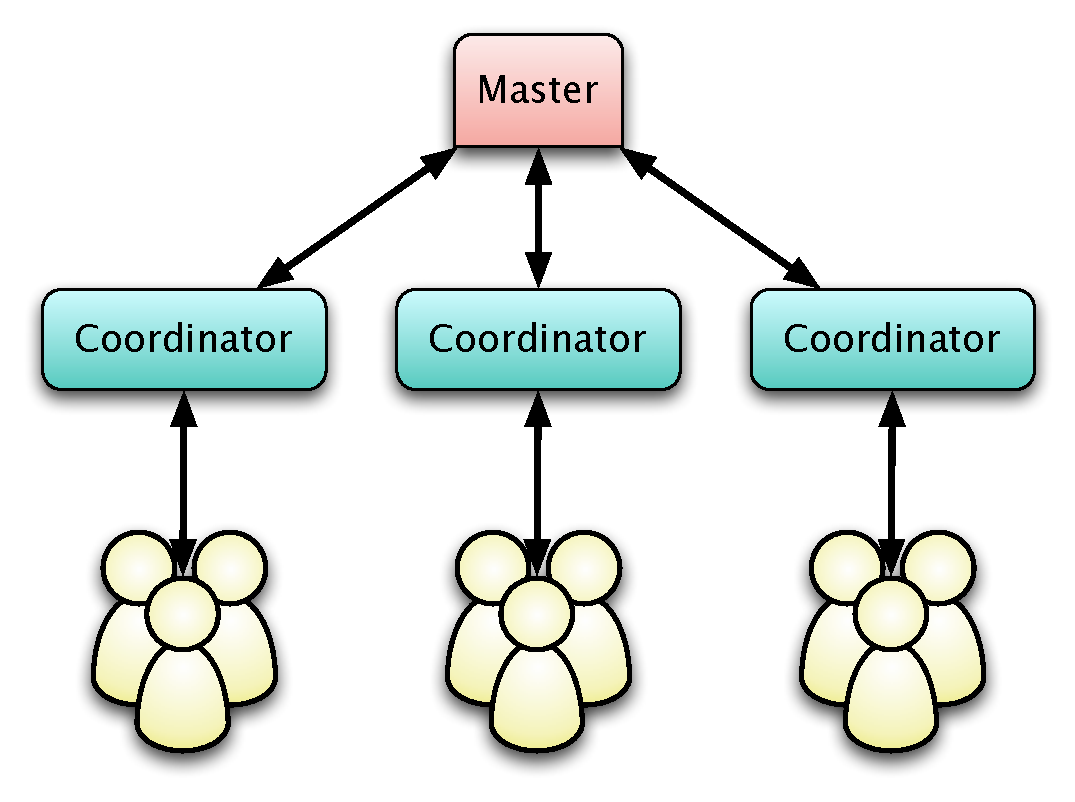
\includegraphics[width=3in]{figures/arch0.pdf}
    \end{center}
    \caption{Basic architecture of the system.}
    \label{arch}
\end{figure*}

In order to support simulations on the scale of millions of agents, Tecellate can be run in a
distributed mode on many machines. Individual components communicate via TCP. The architecture of
this distributed version is shown in figure \ref{arch}.

\begin{figure*}
    \begin{center}
        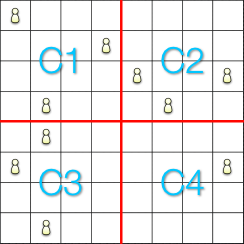
\includegraphics[width=3in]{figures/arch1.png}
    \end{center}
    \caption{Grid-based method for distributing work across coordinators}
    \label{geoarch}
\end{figure*}

Agents are run in individual processes. In order to interact with the simulation, they connect to a
\textbf{coordinator}. Coordinators are responsible for evaluating discrete grid sections each turn
and communicating their results to each other when relevant. The organization of a square grid
section is shown in figure \ref{geoarch}.

The simulation starts with all agent and coordinator processes waiting and listening at individual
addresses. A master process reads a configuration file with their addresses and initial states,
sends information about how to connect to each other, waits for the connections to finish, and
instructs the coordinators to begin the simulation. It then exits and the other processes log
simulation data to configurable log files.

Each coordinator is responsible for a rectangular section of the grid. These sections are assigned
at the start of the simulation and do not change. Coordinators are connected with neighbor
coordinators that share adjacent grid sections. When an agent moves from one grid section to
another, the agent connects to the coordinator responsible for the new section.

\subsection{Coordinator Implementation Details}

There are two main types of threads associated with each coordinator. One kind of thread (A-thread) requests agent data from neighbors, and then applies the simulation rules to the agents's previous states based on their requested actions and the states of the agents at the neighbor coordinators. There is only one of these threads. The other kind of thread (B-thread) serves requests for agent information from neighbors, and there is one of these for each neighbor ($|N|$).

The A-thread and the B-threads communicate using two semaphores, \textbf{turnAvailable} and \textbf{requestsServed}. The A-thread signals \textbf{turnAvailable} $|N|$ times when a turn has been processed, and the B-threads each wait on it before serving a new request. When a B-thread has served a request, it signals \textbf{requestsServed}. The A-thread waits on \textbf{requestsServed} before it begins processing a new turn to avoid overwriting data that B-threads are still serving. The system starts with \textbf{turnAvailable} unlocked for the B-threads.

This system allows processing and RPC serving to run in parallel, with processing running one step ahead of RPC serving.

\subsection{Issues and Possible Improvements}

This problem could be solved by allowing the master process to dynamically reallocate the space
assigned to each coordinator. \textbf{This dynamic reassignment is very similar to the problem of
assigning many application instances to many servers,} but in addition to simply trying to
distribute CPU and memory load evenly, we are also trying to reduce the traffic between servers
which must pass data to each other (agent broadcasts) for the simulation to be correct.
